%Command-----------------------------------------------------
\rhead{\Large 12 Thì Trong Tiếng Anh}
\title{\Huge \textbf{12 Thì \\ Trong Tiếng Anh}}

\maketitle
\tableofcontents
\newcommand{\structure}[3]{
    \newcolbox{Structure}{
        \begin{tabular}{l|l}
            \green{(+)}&#1\\
            \red{(-)}&#2\\
            \yellow{(?)}&#3\\
        \end{tabular}
    }
}
\newcommand{\dStructure}[6]{
    \newcolbox{Structure}{
        \begin{tabular}{l|l}
            \green{(+)}&#1\\
            \red{(-)}&#2\\
            \yellow{(?)}&#3\\
            \hline
            \green{(+)}&#4\\
            \red{(-)}&#5\\
            \yellow{(?)}&#6\\
        \end{tabular}
    }
}

%Overview---------------------------------------------------
\chapter{Overview}
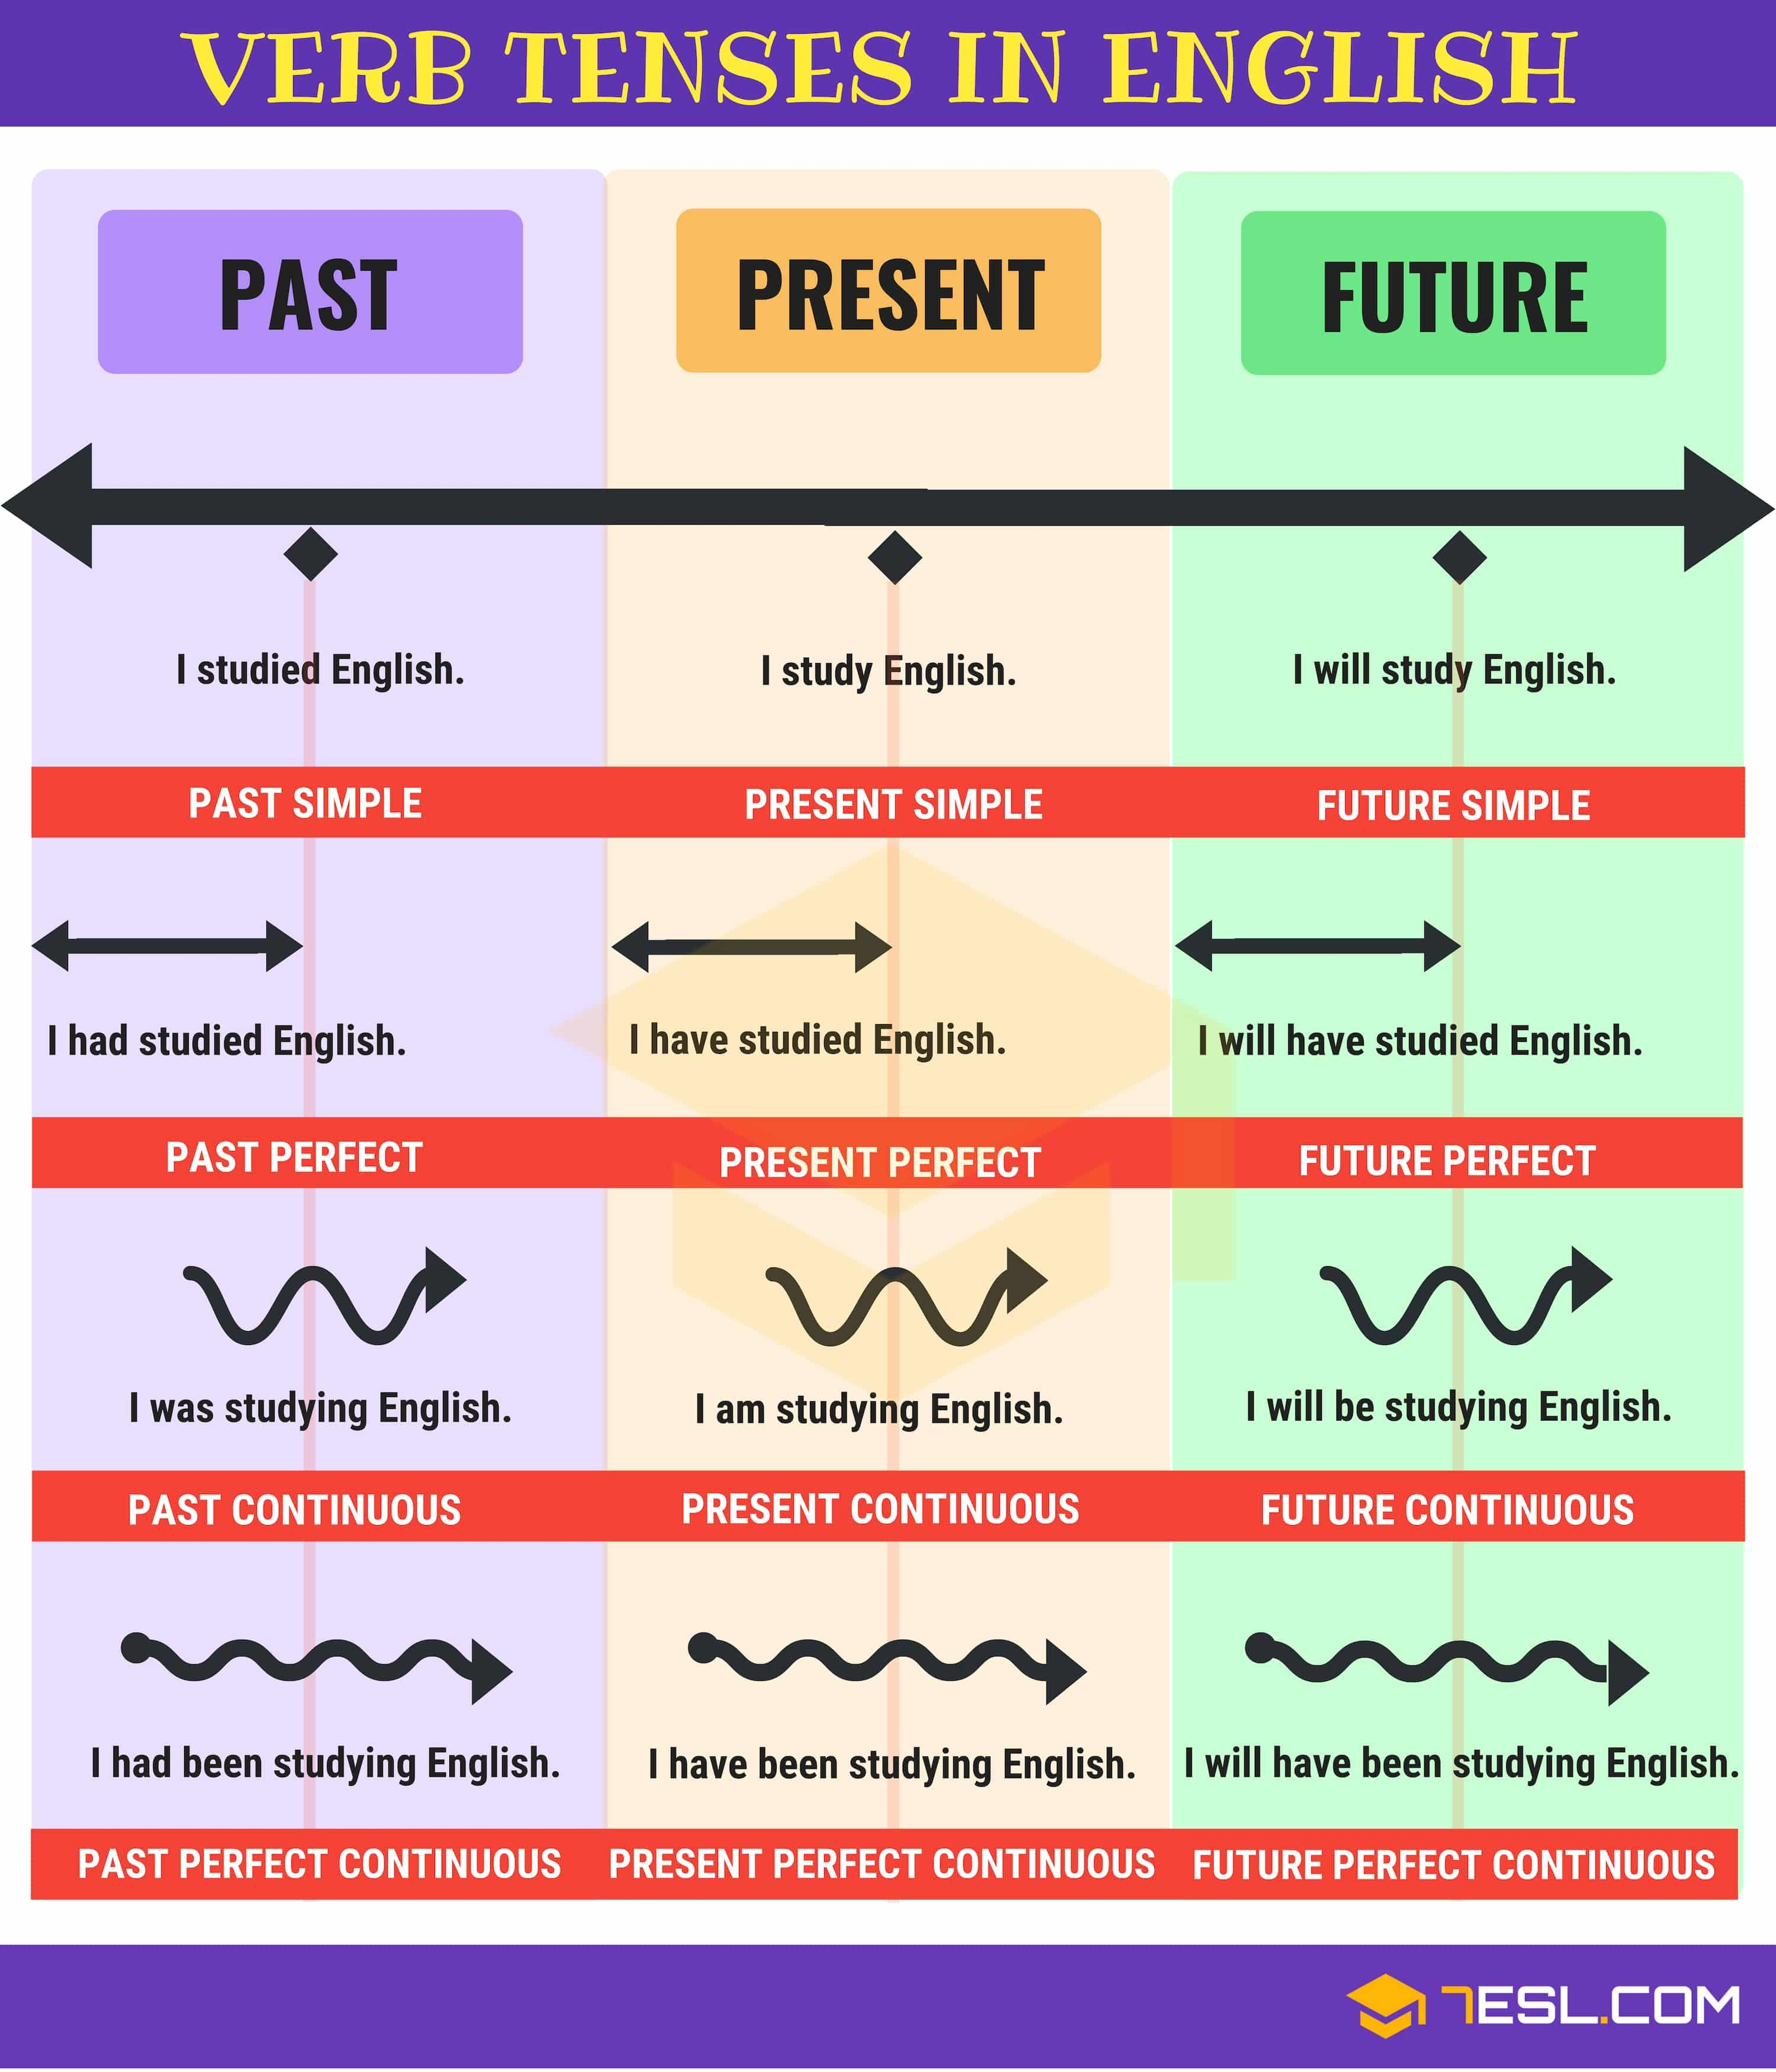
\includegraphics[width=\textwidth]{project-folders/12Tenses/englishTensesOverView.jpg} 

\vspace*{-1\textheight}
\newpage
\centering
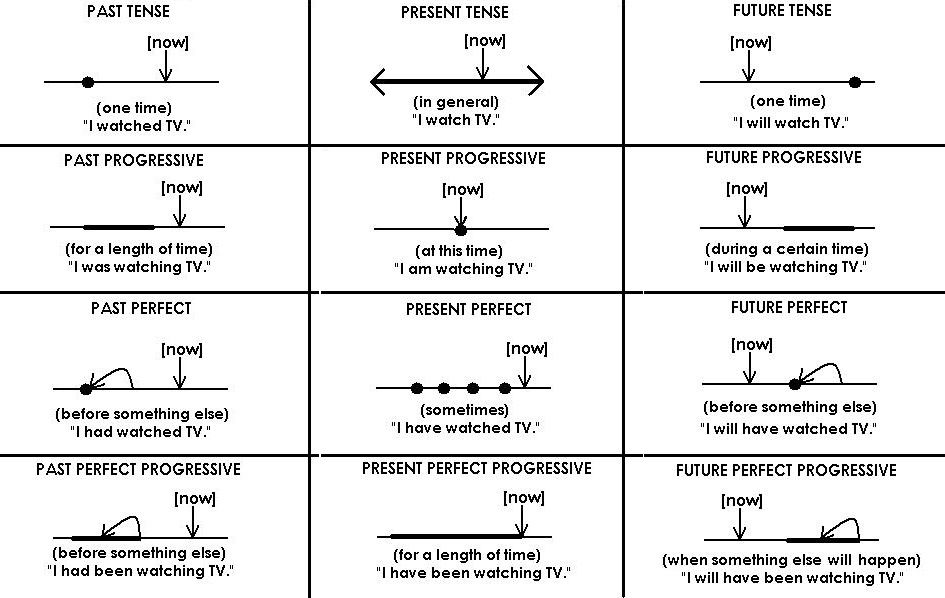
\includegraphics[width=\textwidth]{project-folders/12Tenses/englishtensesoverview2.jpg}\\\vspace{1cm}
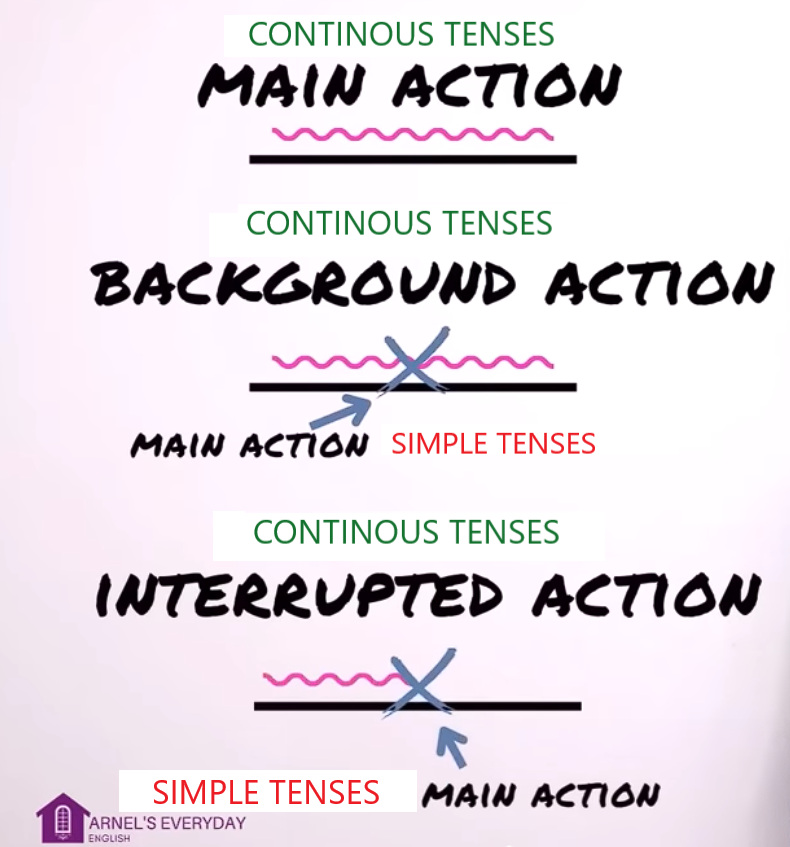
\includegraphics[scale=0.5]{project-folders/12Tenses/actions.png}
%Attention----------------------------------------------------
\chapter{Attention!}
\newcolbox{}{
    \begin{enumerate}
        \item Stative Verbs Are Not Used In Continous/Progressive Tenses
        \item The Perfect Tenses Emphasize The Result And Number Of Times An Action Is Performed
        \item The Perfect Continous Tenses Emphasize The Continuity And Duration Of The Action
        \item Past Simple, Continous And Future Simple, Continous Need A Specific Time
    \end{enumerate}
}
%Past----------------------------------------
\chapter{Past}
\section{Past Simple}
\dStructure{
    S + V\udsc{2} + O}{
    S + Did + Not + V + O}{
    Did + S + V + O?}{
    S + \red{BE} + O}{
    S + \red{BE} + Not + O}{
    \red{BE} + S + O?
}
\newcolbox{Usage}{
    \begin{enumerate}
        \item Actions That Started And Finished In The Past
    \end{enumerate}
}

\section{Past Continous}
\structure{
    S + \red{BE} + V\udsc{ing} + O}{
    S + \red{BE} + Not + V\udsc{ing} + O}{
    \red{BE} + S + V\udsc{ing} + O?
}
\newcolbox{Usage}{
    \begin{enumerate}
        \item Actions That Were Continuing At A Specific Time In The Past\\
        
        \hrule
        \item Parallel Actions
    \end{enumerate}
}

\section{Past Perfect}
\dStructure{
    S + Had + V\udsc{3} + O}{
    S + Had + Not + V\udsc{3} + O}{
    Had + S + V\udsc{3} + O?}{
    S + Had + Been + O}{
    S + Had + Not + Been + O}{
    Had + S + Been + O?
}

\newcolbox{Usage}{
    \begin{enumerate}
        \item Actions That Completed/Not Completed At A Nonspecific Point In The Past
        \item Actions That Started And Lasted Or Finished Before Another Action In The Past\\
        \hrule
        \item Actions Has Already Occurred But The Result Is Still Relevant To The Present
    \end{enumerate}
}
\section{Past Perfect Continous}
\structure{
    S + Had + Been + V\udsc{ing} + O}{
    S + Had + Not + Been + V\udsc{ing} + O}{
    Had + S + Been + V\udsc{ing}?
}
\newcolbox{Usage}{
    \begin{enumerate}
        \item Actions That Started And Lasted Or Finished Before Another Action In The Past\\
        \hrule
        \item Actions That Occurred To Preparation For Another Action
        \item Actions Has Already Occurred But The Result Is Still Relevant To The Present
    \end{enumerate}
}
%Present--------------------------------------------------
\chapter{Present}
\section{Present Simple}
\dStructure{
    S + V\udsc{1} + O}{
    S + Do/Does + V + O}{
    Do/Does + S + V + O?}{
    S + \red{BE} + O}{
    S + \red{BE} + Not + O}{
    \red{BE} + S + O?
}

\newcolbox{Usage}{
    \begin{enumerate}
        \item General Facts
        \item Regular Actions\\
        \hrule
        \item Schedules
    \end{enumerate}
}

\section{Present Continous}
\structure{
    S + \red{BE} + V\udsc{ing} + O}{
    S + \red{BE} + Not + V\udsc{ing} + O}{
    \red{BE} + S + V\udsc{ing} + O?
}
\newcolbox{Usage}{
    \begin{enumerate}
        \item Continuing Actions (Now)\\
        \hrule
        \item One-Time Actions
        \item Repeated Actions That Make Discomfort
        \item Definitely-Impending Actions In The Near Future
    \end{enumerate}
}

\section{Present Perfect}
\dStructure{
    S + Have/Has + V\udsc{3} + O}{
    S + Have/Has + Not + V\udsc{3} + O}{
    Have/Has + S + V\udsc{3} + O?}{
    S + Have/Has + Been + O}{
    S + Have/Has + Not + Been + O}{
    Have/Has + S + Been + O?
}
\newcolbox{Usage}{
    \begin{enumerate}
        \item Actions That Started In The Past, Continue Into The Present And Can Continue Into The Future\\
        \hrule
        \item General Life Experience
        \item Actions Just Happened
        \item In-Past Actions But Important At Speaking Moment
    \end{enumerate}
}

\section{Present Perfect Continous}
\structure{
    S + Have/Has + Been + V\udsc{ing} + O}{
    S + Have/Has + Not + Been + V\udsc{ing} + O}{
    Have/Has + S + Been + V\udsc{ing} + O?
}
\newcolbox{Usage}{
    \begin{enumerate}
        \item Actions That Started In The Past And Still Continue In The Present
    \end{enumerate}
}

%Future--------------------------------------
\chapter{Future}
\section{Future Simple}
\dStructure{
    S + Will + V + O}{
    S + Will + Not + V + O}{
    Will + S + V + O?}{
    S + Will + be + O}{
    S + Will + Not + be + O}{
    Will + S + be + O?
}
\newcolbox{Usage}{
    \begin{enumerate}
        \item Actions In The Future
    \end{enumerate}
}

\section{Future Continuous}
\structure{
    S + Will + be + V\udsc{ing} + O}{
    S + Will + Not + be + V\udsc{ing} + O}{
    Will + S + be + V\udsc{ing} + O?
}
\newcolbox{Usage}{
    \begin{enumerate}
        \item Actions Will Be Happening In The Future\\
        \hrule
        \item Actions That Is Happening Will Be Interrupted By Another Action In The Future
    \end{enumerate}
}

\section{Future Perfect}
\dStructure{
    S + Will + Have + V\udsc{3} + O}{
    S + Will + Not + Have + V\udsc{3} + O}{
    Will + S + Have + V\udsc{3} + O?}{
    S + Will + Have + Been + O}{
    S + Will + Not + Have + Been + O}{
    Will + S + Have + Been + O?
}
\newcolbox{Usage}{
    \begin{enumerate}
        \item Ations That Completed Before Another Action In The Future
    \end{enumerate}
}

\section{Future Perfect Continous}
\structure{
    S + Will + Have + Been + V\udsc{ing} + O}{
    S + Will + Not + Have + Been + V\udsc{ing} + O}{
    Will + S + Have + Been + V\udsc{ing} + O?
}
\newcolbox{Usage}{
    \begin{enumerate}
        \item Actions That Completed Before Another Action In The Future
    \end{enumerate}
}